\documentclass[sigplan]{acmart}

\settopmatter{printacmref=false} % Removes citation information below abstract
\renewcommand\footnotetextcopyrightpermission[1]{} % removes footnote with conference information in first column
\pagestyle{plain} % removes running headers

\usepackage[english]{babel}
\usepackage{listings}
\usepackage{url}

\begin{document}

\title{Implementation of Cholesky Factorization using Intel AVX insructions}

\author{Oleksandr Zaytsev}
\affiliation{%
  \institution{Ukrainian Catholic University\\
  Faculty of Applied Sciences}
  \city{Lviv}
  \state{Ukraine}
}
\email{oleks@ucu.edu.ua}

\begin{abstract}
Intel Advanced Vector Extensions (Intel AVX) is a set of instructions for doing Single Instruction Multiple Data (SIMD) operations on Intel architecture CPU\cite{lomont-11}.

In this work I demonstrate how AVX instructions can be used to speed up the execution of widely used numerical algorithms. Cholesky factorization was chosen as an example due to it importance.
\end{abstract}

\keywords{SIMD, AVX, parallel algorithms, numerical methods, Cholesky factorization}

\maketitle

\section{Introduction}
Software packages like R call native functions from LAPACK etc.

\subsection{Cholesky Factorization}
Every symmetric positive-definite matrix $A$ can be decomposed into the product

\[ A = LL^\top \]

Where $L$ is a lower-triandular matrix.

\section{Data generation}
I used R to generate 6 symmetric positive-definite matrices with real-value entries. The matrices are square and have the following $250, 500, 1000, 2500, 5000, 7500$ rows respectively. These matrices are then stored in binary files and loaded by other modules of this project.

I chose the approach of pre-generated matrices as opposed to the idea of generating a new matrix for each experiment, because this way the measurements will be more accurate. I compare the performance of two algorithms on exactly the same input.

\section{Implementation}

\lstset {language=C++}
\begin{lstlisting}
double sum;
__m256d ax = _mm256_loadu_pd(&a[0]);
__m256d bx = _mm256_loadu_pd(&b[0]);
__m256d cx = _mm256_mul_pd(ax, bx);
__m256d hsum = _mm256_add_pd(cx,
    _mm256_permute2f128_pd(cx, cx, 0x1));
_mm_store_sd(&sum,
    _mm_hadd_pd(
        _mm256_castpd256_pd128(hsum),
        _mm256_castpd256_pd128(hsum)));
\end{lstlisting}

\section{Experimental results}

The main hypothesis is that generative adversarial networks with reinforcement learning based generator, when applied to the

\begin{figure}[H]
  \begin{center}
  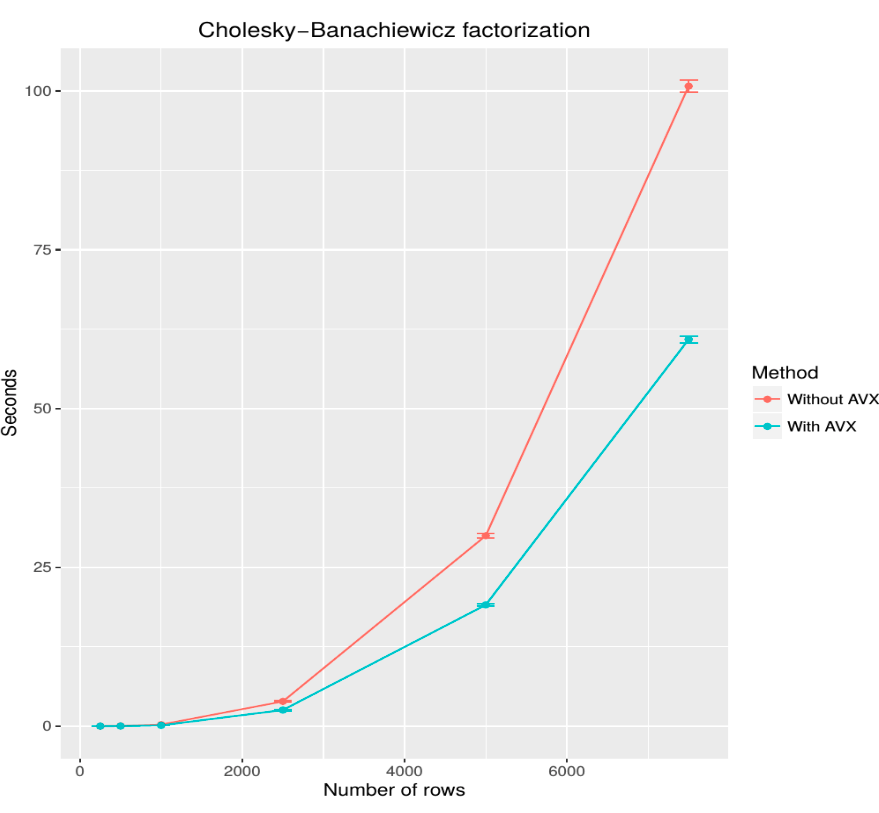
\includegraphics[width=\linewidth]{img/experiment}
  \caption{Comparing the performance of two algorithms}
  \end{center}
\end{figure}

problem of abstractive scientific text summarization, can provide better results than recent state-of-the-art approaches. 

\section{Related work}

Allahyari et al.\cite{allahyari-17} make a survey of the most successful text summarization techniques as of July 2017.

This September Li et al. \cite{li-cohn-17} described their submission to the sentiment analysis sub-task of ?Build It, Break It: The Language Edition (BIBI)? where they successfully apply generative approach to the problem of sentiment analysis.

In their paper \textit{Generative Adversarial Network for Abstractive Text Summarization} Liu et al.\cite{liu-17} built an adversarial model that achieved competitive ROUGE scores with the state-of-the-art methods on CNN/Daily Mail dataset. They compare the performance of their approach with three methods, including the abstractive model, the pointer-generator coverage networks, and the abstractive deep reinforced model.

In contrast Zhang et al.\cite{zhang-17} don't use reinforcement learning but rather introduce TextGAN with an LSTM-based generator and kernelized discrepancy metric.

% \section{Research design and methods}

% We will be applying existing discrete GANs to the data collected from arXiv. One of the lates successful models  for scientific text summarization will be selected as our baseline.

\section{Data collection and preparation}

arXiv provides a RESTful API\footnote{\url{https://arxiv.org/help/api/index}} that allows us to search for papers from a specific category and inside a specific time range. The results are returned as an HTML page which can be easily parsed.

\paragraph{Collecting paper IDs} We started by making requests to arXiv and parsing the response to acquire unique identifiers of each paper. These are the fixed-length strings that look like this: \textbf{1801.01587}. They allow us to access everything related to this paper (including its metadata and full text as PDF). We have only collected 2000 IDs from stat.ML category. We didn't collect all the papers because of network restrictions of arXiv API, huge amount of space required to store them, and the time required to process them. We might create a larger database of papers till the second evaluations, but for now a sample of 2000 random papers from one category will be enough.

\paragraph{Collecting abstracts} Having the list of paper IDs it was no trouble to make 2000 requests to the API and collect abstracts of these papers in plain text form. To get the full text of a paper we must parse its PDF, which can introduce noise and loose peces of text. So being able to collect abstracts directly from arXiv greatly simplifies the task.

\paragraph{Downloading PDF files} The same way as we did it with abstracts, we were able to construct URLs using paper IDs, and donload each paper using wget tool.

\paragraph{Extracting text from PDF} Extracting text from PDF is a complicated task. We used a python binding to Apache Tika\footnote{\url{https://github.com/chrismattmann/tika-python}} to parse the PDF files. The extracted text contained many special characters (noise) which had to be removed manually. 

\paragraph{Cleaning the text} After removing special characters produced by Tika, we also had to remove all mathematical expressions because the can not be parsed into plain text and Tika just turns an expression like this $y = f(x)$ into something like \textit{y f x} or \textit{ytx}. More complex expressions (like sums, integrals etc.) produced much more noise, and it was very hard to identify and remove it. We wanted to remove everething that is not a known English word. But that would filter out words like "GAN", "backprop" etc. So we filtered the words based on their length and frequence of vowels. That leaves some noise, but it shouldn't cause too much damage to our model (at least less damage than would be caused by removing the word "GAN"). Hopefully, we will come up with a more ellegant solution by the time of second evaluations.

\paragraph{} As a result, we have created a database of 2000 papers. For each of these papers we store its name, a list of authors, full text without an abstract, and abstract stored in a separate column. 

\section{Baseline models}

As a baselin model we selected a seq2seq model with deep LSTM\cite{sutskever-17} together with beam search and attention. At this point it is too hard to produce an abstract from the text of a paper, so we started with a simpler task of generating a title from the text of an abstract. We represented each absract as a numeric vector using word embedings and fed it to the model together with a corresponding title. After some training our model was able to generate meaningful titles for most abstracts. Take a look at this example:

\paragraph{Abstract} this is great popcorn and i too have the whirly pop. the unk packs work wonderfully. i have not found it too salty or the packages leak. i have found the recent price of \$35 too expensive and have purchased direct from great american for half the price.

\paragraph{Predicted summary} great popcorn!!

\paragraph{Actual summary} great unk american popcorn

\paragraph{} It is not clear yet if we will be able to produce abstracts based on the whole text of an article. Such problems have very big feature space which might overcomplicate our task. So on the next stage of our project we will continue generating titles from abstracts and try doing that with discrete GANs. If our experiments prove to be successful, we will try scaling up to full texts of papers in our dataset.

% \subsection{Timeframes}

% \paragraph{Deliverables for the $1^{st}$ evaluation}
% \begin{itemize}
% \item Dataset of papers collected from arXiv
% \item Results of feature extraction
% \item Implementations of the baseline state-of-the-art model and its application to our dataset
% \end{itemize}

% \paragraph{Deliverables for the $2^{nd}$ (final) evaluation}
% \begin{itemize}
% \item Implementation of several discrete GAN models
% \item Evaluation of the created models on our dataset
% \item Paper describing the results of our research
% \end{itemize}

\section{Strength and weakness of the study}
GANs have proved to be the most successful when it comes to generative images, but their application to the problems of the text generation is not well studied. So we expect our research to introduce novel approaches and original ideas that may advance the field of natural language processing.
However, there are high risks that this approach may not give good results at all, because there are still lots of issues about  usage of neural networks with language data. The other possible weakness is a difficulty to compare the results with other papers, as there are not a lot of researches concerning this or relative subject. 
We are also currently looking for supervisors who might be interested in the following topic, so we could have a mentorship during the research.

\bibliographystyle{alpha}
\bibliography{CholeskyAVX}

\end{document}